% mnras_template.tex 
%
% LaTeX template for creating an MNRAS paper
%
% v3.0 released 14 May 2015
% (version numbers match those of mnras.cls)
%
% Copyright (C) Royal Astronomical Society 2015
% Authors:
% Keith T. Smith (Royal Astronomical Society)

% Change log
%
% v3.0 May 2015
%    Renamed to match the new package name
%    Version number matches mnras.cls
%    A few minor tweaks to wording
% v1.0 September 2013
%    Beta testing only - never publicly released
%    First version: a simple (ish) template for creating an MNRAS paper

%%%%%%%%%%%%%%%%%%%%%%%%%%%%%%%%%%%%%%%%%%%%%%%%%%
% Basic setup. Most papers should leave these options alone.
\documentclass[fleqn,usenatbib]{mnras}

% MNRAS is set in Times font. If you don't have this installed (most LaTeX
% installations will be fine) or prefer the old Computer Modern fonts, comment
% out the following line
% Depending on your LaTeX fonts installation, you might get better results with one of these:
% \usepackage{mathptmx}
% \usepackage{txfonts}

% Use vector fonts, so it zooms properly in on-screen viewing software
% Don't change these lines unless you know what you are doing
\usepackage[T1]{fontenc}

% Allow "Thomas van Noord" and "Simon de Laguarde" and alike to be sorted by "N" and "L" etc. in the bibliography.
% Write the name in the bibliography as "\VAN{Noord}{Van}{van} Noord, Thomas"
\DeclareRobustCommand{\VAN}[3]{#2}
\let\VANthebibliography\thebibliography
\def\thebibliography{\DeclareRobustCommand{\VAN}[3]{##3}\VANthebibliography}


%%%%% AUTHORS - PLACE YOUR OWN PACKAGES HERE %%%%%

% Only include extra packages if you really need them. Common packages are:
\usepackage{graphicx}	% Including figure files
\usepackage{amsmath}	% Advanced maths commands
\usepackage{amssymb}	% Extra maths symbols
\usepackage{newtxtext,newtxmath}

%%%%%%%%%%%%%%%%%%%%%%%%%%%%%%%%%%%%%%%%%%%%%%%%%%

%%%%% AUTHORS - PLACE YOUR OWN COMMANDS HERE %%%%%

% Packages for slightly better tables
\usepackage{booktabs}
% SI units package
\usepackage{siunitx} % Better units, especially SI
% Units used in work
\DeclareSIUnit[]\solarmass
{\text{\ensuremath{\textup{M}_{\odot}}}}
\DeclareSIUnit[]\solarluminosity
{\text{\ensuremath{\textup{L}_{\odot}}}}
\DeclareSIUnit[]\solarradius
{\text{\ensuremath{\textup{R}_{\odot}}}}
\DeclareSIUnit[]\year
{\text{yr}}
\DeclareSIUnit[]\au
{\text{AU}}
\DeclareSIUnit[]\parsec
{\text{pc}}
\DeclareSIUnit[]\erg
{\text{erg}}
\DeclareSIUnit[]\arcsecond
{\text{as}}

% Author commands
\newcommand{\ts}{\textsuperscript}

% Math macros 
\newcommand{\swr}{\ensuremath{_{\text{WR}}}}
\newcommand{\sob}{\ensuremath{_{\text{OB}}}}
\newcommand{\rms}[1]{\ensuremath{_{\text{#1}}}}

% Please keep new commands to a minimum, and use \newcommand not \def to avoid
% overwriting existing commands. Example:
%\newcommand{\pcm}{\,cm$^{-2}$}	% per cm-squared

%%%%%%%%%%%%%%%%%%%%%%%%%%%%%%%%%%%%%%%%%%%%%%%%%%

%%%%%%%%%%%%%%%%%%% TITLE PAGE %%%%%%%%%%%%%%%%%%%

% Title of the paper, and the short title which is used in the headers.
% Keep the title short and informative.
\title[Hydrodynamical Simulation of WR140]{Exploring dust formation in the episodic WCd system WR140}

% The list of authors, and the short list which is used in the headers.
% If you need two or more lines of authors, add an extra line using \newauthor
\author[J. W. Eatson et al.]{
J. W. Eatson\thanks{E-mail: \href{mailto:py13je@leeds.ac.uk}{py13je@leeds.ac.uk}} \&
J. M. Pittard
\\
School of Physics and Astronomy, University of
       Leeds, Woodhouse Lane, Leeds LS2 9JT, UK\\  
}

% These dates will be filled out by the publisher
\date{Accepted XXX. Received YYY; in original form ZZZ}

% Enter the current year, for the copyright statements etc.
\pubyear{2022}

% Don't change these lines
\begin{document}
\label{firstpage}
\pagerange{\pageref{firstpage}--\pageref{lastpage}}
\maketitle

% Abstract of the paper
\begin{abstract}
\noindent


\end{abstract}

% Select between one and six entries from the list of approved keywords.
% Don't make up new ones.
\begin{keywords}
stars: Wolf-Rayet -- methods: numerical -- binaries: general
\end{keywords}

%%%%%%%%%%%%%%%%%%%%%%%%%%%%%%%%%%%%%%%%%%%%%%%%%%

%%%%%%%%%%%%%%%%% BODY OF PAPER %%%%%%%%%%%%%%%%%%

\section{Introduction}

The dynamics of massive stars in binary systems is a particularly fascinating subject.
These incredibly violent systems are obscured behind vast clouds of outflowing stellar wind, the result of the most massive stars we know of slowly tearing themselves asunder.
Despite powerful winds, extreme temperatures, and intense astrophysical shocks from these colliding winds, interstellar dust

% Observational history, define acronyms commonly used


% Dust production yields

In fact, these dust producing CWB (WCd) systems can produce an extreme quantity of dust.
Typically around $1\%$ of the stellar wind is converted into dust a short amount of time after wind collision, but in the case of more prolific systems such as WR104 this can be as high as $36\%$ \citep{lauRevisitingImpactDust2020}.
This corresponds to dust production rates on the order of $10^{-6} \, \si{\solarmass\per\year}$, rivalling other profuse dust producing phenomena such as AGB stars.

% Difficulty of detailed observation
While we know that truly colossal amounts of dust form in these systems through infrared observation, we find that the mechanisms involved in 

% Dust formation particulars
% Dust forms in wcr
Observations conclude that dust forms exclusively within the WCR of the system,
% Dust forms close to system
observations also indicate that dust formation occurs rapidly and close to the system
\citep{williamsInfraredPhotometryLatetype1987,williamsMultifrequencyVariationsWolfrayet1990},

this is further backed up by grain 

% Bringing it all together, theories as to how dust formation occurs, density, shielding etc.

% What we intend to do in this project

In this paper we will discuss our methodology in section 

\section{Methodology}
\label{sec:paper-2-methodology}


The periodic dust forming system WR140 was simulated using a fork of the Athena++ hydrodynamical code \citep{stoneAthenaAdaptiveMesh2020}, a series of modifications were implemented to simulate binary system orbits, stellar wind outflows and dust evolution.
These simulations were conducted in 3D in a Cartesian co-ordinate system.
The code solves a Riemann problem at each cell interface to determine the time-averaged values at the zone interfaces, and then solves the equations of hydrodynamics:

\begin{subequations}
  \begin{align}
    \frac{\partial\rho}{\partial t}+\nabla \cdot \left(\rho \boldsymbol{u}\right) & = 0 , \\
    \frac{\partial \rho \boldsymbol{u}}{\partial t} + \nabla \cdot \left(\rho \boldsymbol{u} u + P \right) & = 0, \\
    \frac{\partial \rho \varepsilon}{\partial t} + \nabla \cdot \left[ \boldsymbol{u} \left( \rho\varepsilon + P \right) \right] & = \dot E_\text{cool} , 
  \end{align}
\end{subequations}

\noindent
where $\varepsilon$ is the total specific energy ($\varepsilon = \boldsymbol{u}^2/2 + e/\rho $, $\rho$) is the mass density, $e$ is the internal energy density, $P$ is the gas pressure and $u$ is the gas velocity.
In order to simulate radiative losses, the parameter $\dot E_\text{cool}$ is included, which is the energy loss rate per unit volume from the fluid due to gas and dust cooling.

Spatial reconstruction using a piecewise linear method was performed, while the time-integration scheme is a third-order accurate, three-stage strong stability preserving Runge-Kutta\footnote{SSPRK (3,3)} method \citep{gottliebHighOrderStrong2009}.
Several passive scalars are utilised to model wind mixing and dust evolution, the scalar values are transported by the fluid, for a given scalar species $i$, the scalar is advected through the scalar through the following equation:

\begin{equation}
  \rho \frac{dC_i}{dt} = \frac{\partial}{\partial t} \left( \rho C_i \right) + \nabla \cdot \left( C_i \rho \mathbf{u} \right) = -\nabla \cdot \mathbf{Q}_i ,  
\end{equation}

where $\mathbf{Q}_i = - \nu_{ps} \rho \nabla C_i$ is the diffusive flux density and $\nu$ is the passive scalar diffusion coefficient \citep{stoneAthenaAdaptiveMesh2020}.

% Cover mapping on winds

Stellar winds are simulated by modifying the density, $\rho_R$, momentum, $p_R$, and energy, $E_R$ in a small region around both stars.
Winds flow from this ``remap'' region at the stars wind terminal velocity, $v^\infty$. Remap zone parameters are calculated with the formulae

\begin{subequations}
  \begin{align}
    \rho_R & = \frac{\dot M}{4 \pi r^2 v_\infty} , \\
    % P_R    & = \frac{\rho_R}{\mu m_H} k_B T_w , \\
    p_R    & = \rho_R v_{r} , \\
    E_R    & = \frac{P_R}{\gamma - 1} + \frac{1}{2} \rho_R v_\infty^2 ,
  \end{align}
\end{subequations}

\noindent
where $P_R$ is the cell pressure, $P_R = \rho_R k_\text{B} T_w / \mu m_\text{H}$, $T_w$ is the wind temperature, $\mu$ is the mean molecular mass, $m_\text{H}$ is the mass of a hydrogen atom, $v_R$ is the wind velocity as it flows radially from the center of the ``remap zone'' and $r$ is the distance from the current cell to the centre of the remap zone.
This method produces radially out-flowing winds from the star with an expected density and velocity.
This method is stable against numerical instability, while also allowing us to precisely control the winds.

Line driving and wind acceleration effects are not simulated, which can result in divergence with the correct wind velocity as stars approach periastron passage.
Instead, winds are instantaneously accelerated to their terminal velocity.
Additionally, influence from either gravitational self-interaction and interaction with the stars gravity wells is not simulated, with the stellar winds assumed to be travelling far in excess of the system escape velocity.

Adaptive Mesh Refinement was considered for this simulation, however a known issue with the Athena++ code prevented this from being possible.
Passive scalars incorporated into the simulation were found to not be conserved along the interfaces between mesh blocks undergoing refinement, this meant that the simulation would behave non-physically (This bug is recorded as issue \#365 on the Athena++ Github repository\footnote{\texttt{\href{https://github.com/PrincetonUniversity/athena/issues/365.}{https://github.com/PrincetonUniversity/athena/issues/365}}}).
A ring of refined cells across the orbital path was considered, but the performance improvements of this method were found to be negligible and not worth pursuing, as the block based refinement method of Athena++ would result in much redundant refinement.
Instead, a static mesh is used, where a region around the stars at $\phi = 0.95$ is refined to the maximum level, with a gradual de-refinement away from this refinement region.

\subsection{Dust model and cooling}

The dust model in this paper simulates dust growth and destruction through collisions between carbon atoms and dust grains. These grains are simulated in the form of advected scalars in each cell in the numerical grid which propagate with the same hydrodynamical rules as the stellar wind; as such dust can be described as co-moving with the interstellar wind. The two scalars in use are $z$, the dust-to-gas mass ratio within the cell, and $a$, the average grain radius. Using these parameters in addition to the local wind parameters, the dust can be adequately described and evolved with time. %//TODO Clean up this sentence 

A number of assumptions are made in this dust model, for instance, the dust grains are assumed to be spherical, with a uniform density of \SI{3.0}{\gram\per\centi\metre\cubed}. Dust grains are assumed to have a single size in a region, as well as a constant number density, as such, this model does not simulate grain agglomeration and fracturing.
Additional mechanisms for dust formation and destruction could also be implemented such as grain-grain agglomeration and photoevaporation.
Furthermore, a multi-fluid model with drag force coupling could also be implemented, however this is beyond the scope of this paper.

Dust is grown through grain accretion using formulae described by \citep{spitzer_jr._physical_2008}. Dust grains grow via collisions with the surrounding gas, as gas accretes onto these grains the associated density is subtracted from the gas density. The growth rate is such that:

%//TODO I have copy-pasted some paragraphs from paper 1, this needs to be fixed up a bit or streamlined. 


\begin{subequations}
  \begin{align}
    \frac{da}{dt} & = \frac{\xi \rho\rms{C} w_\text{C}}{4 \rho\rms{gr}} , \\
    \frac{dm\rms{gr}}{dt} & = 4\pi \rho\rms{gr} \frac{da}{dt} a^2 = \pi \xi \rho\rms{C} w\rms{C} a^2, \\
    \frac{d\rho\rms{d}}{dt} & = \frac{dm\rms{gr}}{dt} n\rms{d} ,
  \end{align}
\end{subequations}

\noindent

\textbf{THIS PART NEEDS FIXING AFTER PAPER 1 SORTED}

where $w_a$ is the Maxwell-Boltzmann distribution RMS velocity, $\xi_a$ is the grain sticking efficiency, $\rho_{Gr}$ is the grain bulk density, $\rho$ is the gas density, $a$ is the dust grain radius, and $n_D$ is the grain number density. For these simulations, the grain sticking factor has been set to $10\%$, while for low temperature collisions a sticking factor of $100\%$ can be proven, grain sticking in a more energetic, hot regime could significantly reduce the probability of sticking. 

Dust destruction is calculated via gas-grain sputtering using the Draine \& Salpeter prescription - a dust grain has a lifespan, $\tau$, which is dependent on the grain radius, 

\begin{equation}
  \frac{da}{dt} = \tau n\rms{g},
\end{equation}

as the grain loses radius proportional to its loss in mass; assuming a spherical grain, the rate of change in mass and radius can be calculated through the following equation:

\begin{subequations}
  \begin{align}
    \frac{d m\rms{gr}}{dt} & = \frac{4}{3} \pi \tau \rho\rms{gr} n\rms{g} a^2 , \\
    \frac{d \rho\rms{d}}{dt} & = \frac{d m\rms{gr}}{dt} n\rms{d}.
  \end{align}
\end{subequations}

\section{WR140 and simulation parameters}
\label{sec:paper2-wr140}

% Discuss importance of WR 140 system

WR 140 was simulated in this paper as it is considered to be the archetypical episodic CWB system, whose infrared dust emission peaks around periastron passage.
WR 140 deviates from WR 98a and WR 104 by having an extremely eccentric orbit, which significantly effects the cooling parameter as the orbit progresses.
Additionally, the minimum value for $\chi$ is significantly larger than the other systems, and hence cooling would be less dominant on the dynamics of the WCR, even at periapsis.
Though these simulations do not calculate wind acceleration due to radiative line driving, both stellar winds are expected to be accelerated close to their terminal wind velocities \citep{lamersIntroductionStellarWinds1999}.
However, this discrepancy should be noted when considering the results of this paper.
% Discuss simulation parameters
Recent improved estimations of the orbital parameters of WR140 by \cite{thomasOrbitStellarMasses2021} were used to calculate the orbital path for these simulations (see Table \ref{tab:wr140systemparameters}).
% Composition
In order to correctly calculate cooling and dust growth, the abundances of hydrogen, helium, and metals, particularly CNO must be included in the simulations parameters.
A typical wind composition for WC stars was assumed for the Wolf-Rayet star, while a solar abundance was assumed for the OB star (Table \ref{tab:p2-abundances}).

\begin{table}
  \centering
  \begin{tabular}{lll}
    \hline
    $\text{M}_\text{WR}$ & \SI{10.31}{\solarmass} & \cite{thomasOrbitStellarMasses2021} \\
    $\text{M}_\text{OB}$ & \SI{29.27}{\solarmass} & \cite{thomasOrbitStellarMasses2021} \\
    $P$ & \SI{7.926}{\year} & \cite{thomasOrbitStellarMasses2021} \\
    $e$ & 0.8993 & \cite{thomasOrbitStellarMasses2021} \\
    $\dot{\text{M}}_\text{WR}$ & \SI{5.6e-5}{\solarmass\per\year} & \cite{williamsMultifrequencyVariationsWolfrayet1990} \\
    $\dot{\text{M}}_\text{WR}$ & \SI{1.6e-6}{\solarmass\per\year} & \cite{williamsMultifrequencyVariationsWolfrayet1990} \\
    $v^\infty_\text{WR}$ & \SI{2.86e3}{\kilo\metre\per\second} & \cite{williamsMultifrequencyVariationsWolfrayet1990} \\
    $v^\infty_\text{OB}$ & \SI{3.20e3}{\kilo\metre\per\second} & \cite{williamsMultifrequencyVariationsWolfrayet1990} \\
    $\eta$ & 0.031 & Calculated \\
    $\chi_\text{min}$ & 2.69 & Calculated \\
    \hline
  \end{tabular}
  \caption[WR140 system parameters]{WR140 system parameters.}
  \label{tab:wr140systemparameters}
\end{table}

\begin{table}
  \centering
  \begin{tabular}{@{}lll@{}}
  \toprule
  \multicolumn{1}{l}{} & \multicolumn{2}{c}{X(E)} \\ \cmidrule(l){2-3} 
   & Solar & WC \\ \midrule
  H & $0.705$ & $0.000$ \\
  He & $0.275$ & $0.546$ \\
  C & $0.003$ & $0.400$ \\
  N & $0.001$ & $0.000$ \\
  O & $0.010$ & $0.050$ \\
  \hline
  \end{tabular}
  \caption[Abundances by mass used for OB and WR stars]{Abundances used for the OB and WR stars being simulated. Other elements are assumed trace when calculating dust emission \citep{williamsSpectraWC9Stars2015}.}
  \label{tab:p2-abundances}
\end{table}

Due to computing limitations, a complete orbit could not be completed without AMR, instead, a section of the systems orbit, corresponding to an orbital phase of $0.95 \leq \Phi \leq 1.10$ was simulated, where $\Phi$ is the orbital phase.
This section represents the period prior to periastron passage, as well as a brief period after periastron
(Fig. \ref{fig:p2-trajectory}).
This represents a period of approximately \num{1.2} years of the systems orbit, and the period where much of the dust forms \citep{crowther_dust_2003}.
The simulation was run with two different numerical integrators, a 3\ts{rd} order accurate Runge-Kutta integrator (\texttt{rk3}) and a 4\ts{th} order accurate, 5-stage, 3 storage register strong stability preserving Runge-Kutta integrator (\texttt{ssprk5\_4})
\citep{ruuthHighOrderStrongStabilityPreservingRungeKutta2005}.
The \texttt{ssprk5\_4} integrator was found to be approximately 60\% slower, but markedly more stable.
Prior to periastron passage the \texttt{rk3} integrator was used for its speed, but increasing numerical instability as the stars grew closer resulted in this proving untenable, and was switched to \texttt{ssprk5\_4}.
Over periastron passage the average time-step was found to reduce by an order of magnitude, resulting in a corresponding increase to simulation time (Fig. \ref{fig:p2-timestep}).
At the most numerically complex portion of the simulation, a Courant number of $C = 0.04$ had to be used instead of the initial value of $C = 0.15$, in order to preserve numerical stability.
As the simulation moved past periastron the Courant number was increased every 24 hours of wall time, until $C$ returned to the initial value.

The simulation was conducted on the ARC4 HPC cluster at the University of Leeds with 128 cores.
The code was compiled using the Intel \texttt{ICPC} compiler using \texttt{AVX512} optimisations and the Intel MPI library.

\begin{figure}
  \centering
  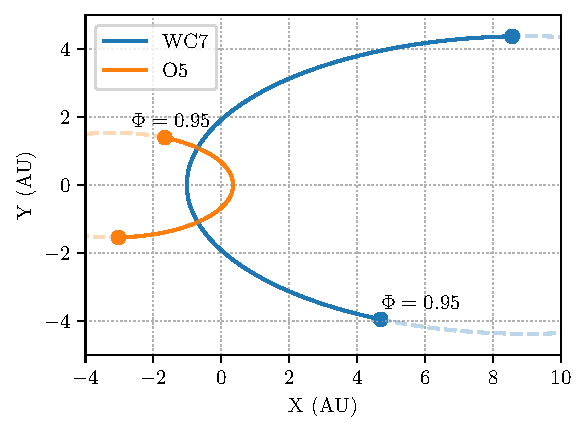
\includegraphics[width=\linewidth]{assets/wr140-path.pdf}
  \caption[Simulation orbital trajectories of WR140 WC7 and O5 stars]{Simulation orbital trajectories of the WC7 and O5 stars in WR140. The solid line represents the orbital phase being simulated, corresponding to $0.95 \leq \Phi \leq 1.10$. The simulation starting position for each star has been annotated.}
  \label{fig:p2-trajectory}
\end{figure}

\begin{figure}
  \centering
  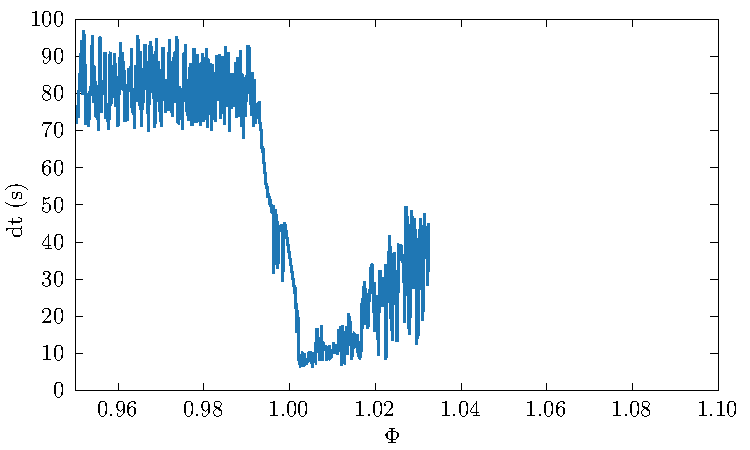
\includegraphics[width=\linewidth]{assets/wr140-dt.pdf}
  \caption[Timestep over WR140 simulation]{Timestep, $dt$, over the course of the WR140 simulation. after periastron passage the \texttt{ssprk5\_4} numerical integrator and a drastically reduced Courant number was adopted in order to preserve numerical stability. This increased simulation time by approximately an order of magnitude.}
  \label{fig:p2-timestep}
\end{figure}

\section{Results}

% Dust production rate

% Instabilities


\section{Conclusion}

\section{Acknowledgements}


%%%%%%%%%%%%%%%%%%%% REFERENCES %%%%%%%%%%%%%%%%%%


\bibliographystyle{mnras}
\bibliography{references.bib} % if your bibtex file is called example.bib

% Don't change these lines
\bsp	% typesetting comment
\label{lastpage}
\end{document}

% End of mnras_template.tex
